\documentclass[a4paper,12pt]{article}

\usepackage{amsfonts}
\usepackage[english]{babel}
\usepackage{float}
\usepackage{fullpage}
\usepackage{graphicx}
\usepackage{listings}
\usepackage{url}

\begin{document}

\title{Reinforcement Learning Agent to Solve 2048 Effectively}
\author{
Robrecht Conjaerts \& Youri Coppens \& Ruben Vereecken \\
Vrije Universiteit Brussel, Pleinlaan 2, 1050 Brussels, Belgium \\
}
\date{\today}
\maketitle

\begin{abstract}
Samenvatting van de paper
\end{abstract}

\section{Introduction}
Since the explosive growth of smartphone usage in our everyday lives, and the improvement of SDK's for smartphone development, we have seen a rapid evolution from software developers to mobile developers. This led to a huge increase of applications for smartphones, with over 1.43 million applications for the Google Play store, and 1.21 million for the Apple App store as of December 2014 \cite{appstores}. One of the more popular applications of 2014, was the puzzle game "2048" \cite{2048}. It is the objective of the player to increase its score by sliding the board (a grid 4x4) such that the same numbers that are next to each other merge, and multiply. These numbers are all powers of 2, and the higher the number gets, the higher your score will be. Figure~\ref{fig:2048} shows what the game looks like after the player has performed a couple of moves. We created an artificial intelligence (AI) that plays the game, and aims to gather a score as high as possible. Using reinforcement learning (RL) \cite{sutton1998rl} we train our agent to learn how to play the game, and how to differentiate between good, and bad actions. This is done by using tile coding \cite{sutton1998rl} to create a feature vector for the state the agent finds itself in, and Q-Learning \cite{sutton1998rl} to update its Q-values. We start the paper by giving background information about the used techniques, and their functionalities. We will then explain in-depth how these methods are integrated in our algorithm, and how they help to learn how to play 2048. We show the results we managed to achieve, and examine them in detail. The paper ends by discussing future possibilities to achieve better results.
\begin{figure}[t]
\centering
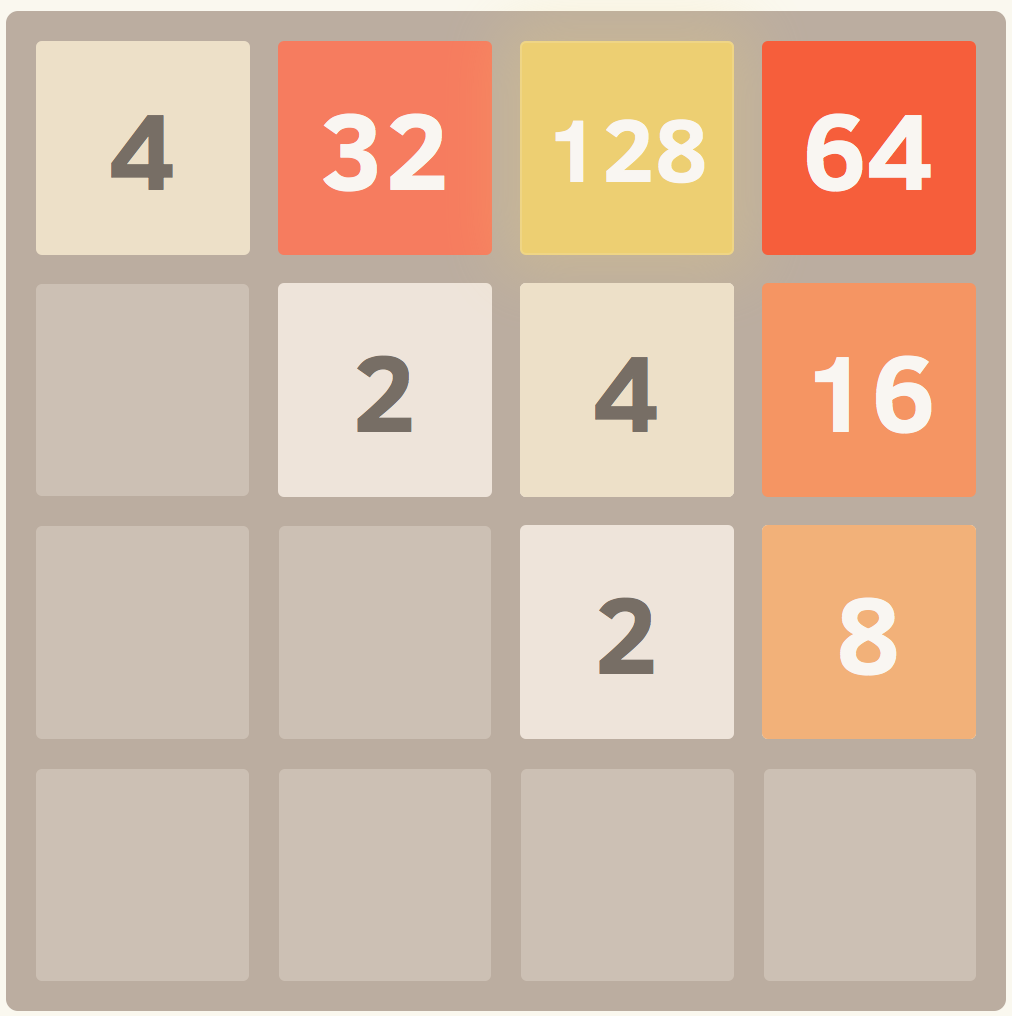
\includegraphics[scale=0.35]{img/2048board}
\caption{The board of 2048, after a couple of moves}
\label{fig:2048}
\end{figure}
\section{Background Information}
This section was created to explain the basics of the techniques we will be using in our algorithm, to help our agent learn how to play the game 2048. 
\subsection{Reinforcement Learning}
When an agent interacts with an environment, and it receives a reward for this action, he will be able to distinguish between good, and bad actions based on this reward. This is what we call reinforcement learning \cite{sutton1998rl}, which we can define as a Markov decision process \cite{howard1960mdp}, that is a 5-tuple $(S, A, P, R, \gamma)$ where:
\begin{itemize}
\item $S$ is a finite set that contains the states of the environment
\item $A$ is a continuous set with actions available in each state
\item $P$ is the probability distribution that assigns a probability to each state, action pair $(S$ x $A) \mapsto [0,1]$
\item $R$ contains the expected immediate rewards (given) for performing an action in a state $(S$ x $A) \mapsto \mathbb{R}$
\item $\gamma$ is the discount factor
\end{itemize}
From the environment an agent will perceive the state $s_{i} \in S$ he is in. Bounded to this state a set of actions $A_{i} \subset A$ that the agent can choose to perform. The agent has a policy $\pi$ that decides which action the agent is going to take. For each state-action pair $(s_{i}, a_{j})$ the agent will receive a reward $r$, and uses this reward to update its policy, such that it will learn how to maximize the cumulative sum of rewards. Thus if we would perform an action $a_{j}$, in a state $s_{i}$, and would be returned a positive reward $r$ the probability of choosing that action $a_{j}$ would increase. The agent does not need to know beforehand which actions are good, and which actions are bad, he learns this by interacting with the environment, and it is in there that the power of RL lies.
\subsubsection{Q-Learning}
One of the best-known algorithms to solve a RL problem is the Q-learning algorithm \cite{sutton1998rl}.
\subsubsection{Generalization and Function Approximation}
\section{Methods}
In detail de methodes bespreken die we gebruiken, de functionaliteiten, eigenschappen en zo
\section{Experimental setup}
Het probleem 2048 goed uitleggen, en als we parameters in onze functies hebben, zeggen waarom die gekozen en zo.
\section{Results}
Resultaten tonen, en bespreken
\section{Discussion and Future work}
Praten over het nut van dit, wat het opgeleverd heeft, en hoe we het kunnen verbeteren in de toekomst
\section{Acknowledgement}

\bibliographystyle{plain}
\bibliography{article}
\end{document}